\begin{figure}[t]
\centering
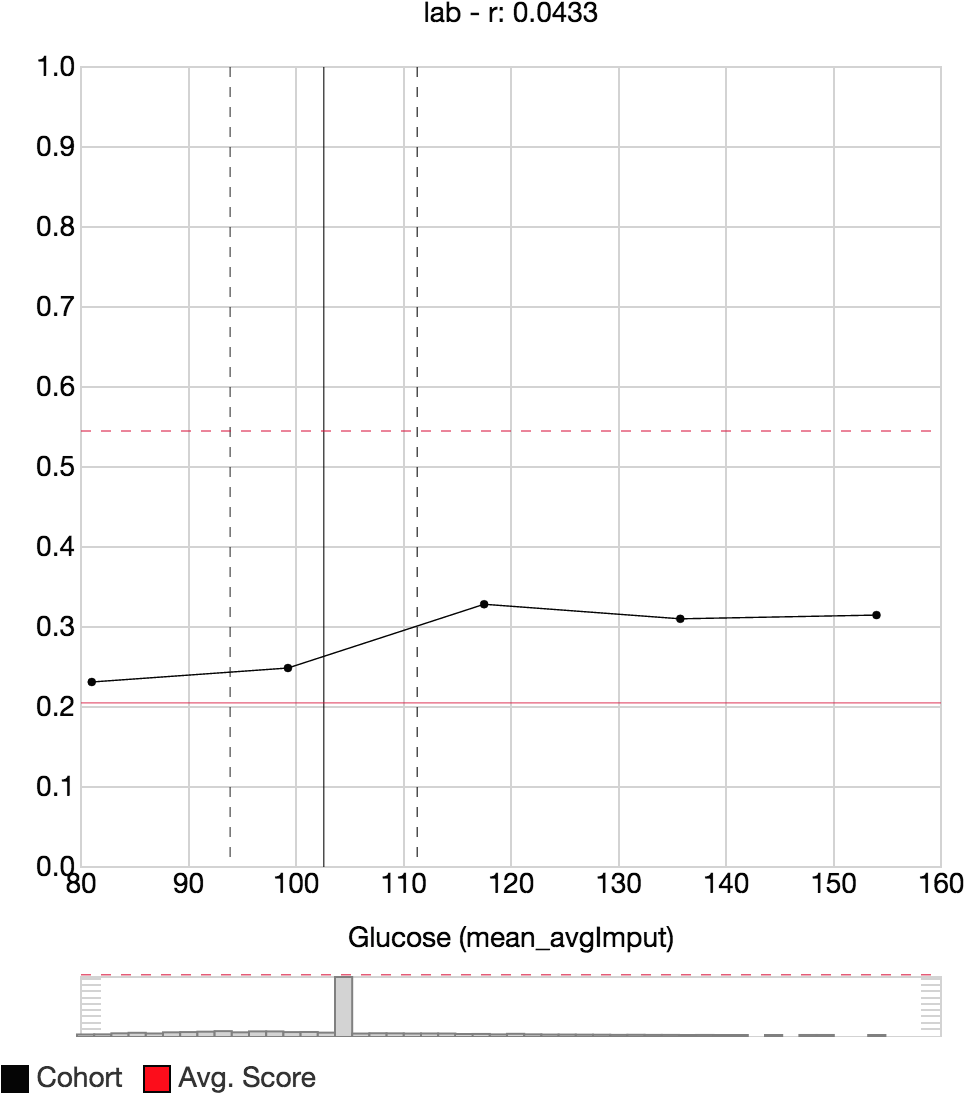
\includegraphics[width=0.3\textwidth]{prospector/sampling_1} % 0.3
~
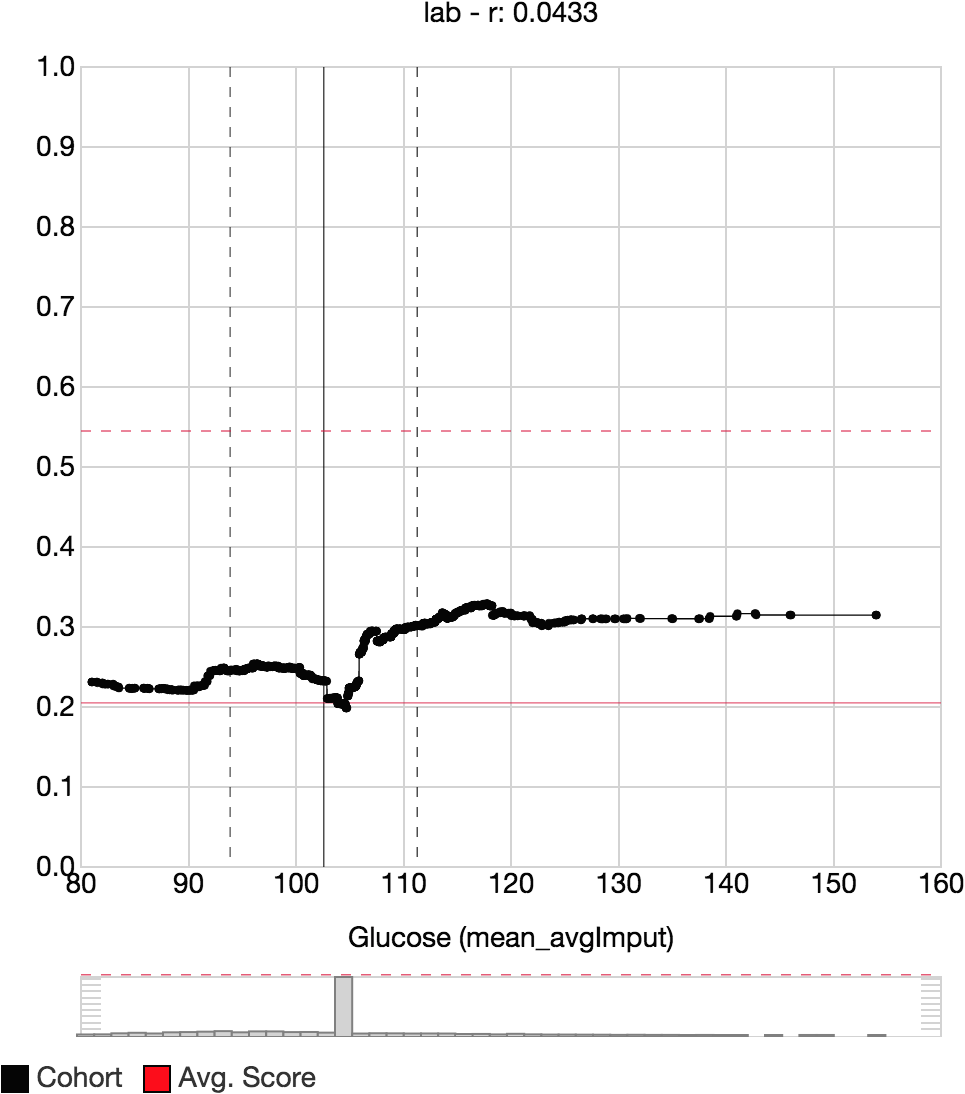
\includegraphics[width=0.3\textwidth]{prospector/sampling_2} % 0.3
~
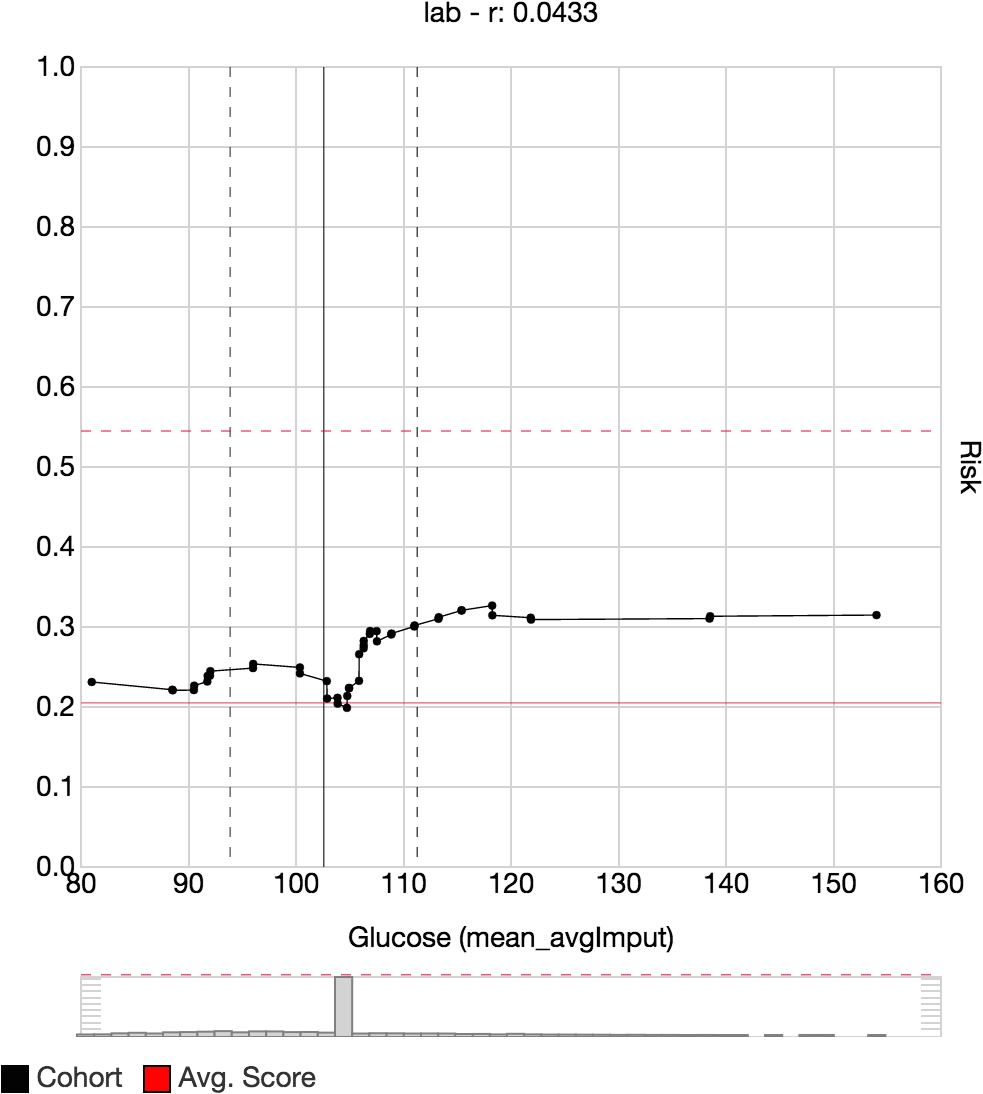
\includegraphics[width=0.3\textwidth]{prospector/sampling_3} % 0.3
\caption[Different sampling strategies for partial dependence plots.]{
Different sampling strategies for partial dependence plots.
The leftmost plot uses a na\"ive sampling which misses the
dip in the predicted risk for a Glucose value around 105.
Using the thresholds of the trees in the random forest
the middle plot shows all details of the displayed model.
The rightmost plot simplifies this by detecting co-linear points
and summarizing them into lines improving readability.
The dip in the predicted risk is due to imputation of missing values
to the mean of the observed values.
This increase in local noise shifts the prediction towards the overall
average predicted risk (the horizontal red line).
Most patients have never had their Glucose value measured.
}
\label{figs:sampling}
\end{figure}